\documentclass{llncs}

\usepackage{graphicx}

\title{Our experience with the\\ CodeContracts static checker \\ 
(Invited Tutorial)}

\author{Francesco Logozzo}
\institute{Microsoft Research, Redmond, WA (USA) \\
\email{logozzo@microsoft.com}
}

\begin{document}
\maketitle
In this tutorial I will report our experience with CodeContracts~\cite{codecontracts}, and in particular with its static checker (cccheck/clousot)~\cite{cccheck}.

CodeContracts are a language-agnostic solution to the specification problem. 
Preconditions, postconditions and object invariants are with opportune method calls acting as specification markers~\cite{embedded-cc-sac-oops-2010}. 
The CodeContracts API is part of the core .NET standard. 
The CodeContracts tools have been downloaded more than 50 000 times, and they are currently used in many projects by professional programmers.

The CodeContracts static checker (cccheck) is designed to be used by non-expert professional programmers, with no background in formal methods, in their every-day development activity. 
The evolution of cccheck is strongly influenced by the user community, who suggest improvements and new features but who also do not hesitate to criticize or stress the tool. 
Because of that, cccheck has a very pragmatic angle, and in many things it is surprisingly different from what one may expect from a purely Academic perspective. 

The main difference of cccheck with respect to similar tools is that is based on abstract interpretation~\cite{CousotCousot77}. 
It focuses on the properties of main interest for the programmer (e.g., non-null values, numerical relationship~\cite{LogozzoFahndrich08,subpolyhedra}, floating point comparisons~\cite{LogozzoFahndrich11}, collection contents~\cite{CousotCousotLogozzo-POPL11}, and simple universally and existential quantifiers \dots). 
It infers loop invariants, preconditions~\cite{CousotCousotLogozzo-VMCAI11}, postconditions, object invariants~\cite{Logozzo-VMCAI07}; it makes explicit the assumptions in the code as the programmer type in her program. 
We found inference to be a crucial point for the adoption of the tool. 
Whereas a strict Design-by-Contract discipline requires the programmer to provide all the annotations, in practice very few of them are willing to pay the burden of the full annotation process. 

In the tutorial I detail the internals of, and the experience with cccheck. 
I report (some of) the user feedback (in the good and the bad). 
I  conclude with a vision of cccheck as a real-time semantic programmer assistant, suggesting semantic code fixes, improving the refactoring  experience (e.g., with the ``extract method with contracts'' refactoring of Fig.~\ref{ExtractMethodWithContracts}), and acting as a discrete, non-intrusive program verifier. 
The verbosity of the warnings can be finely tuned and only a certain class of warnings can be shown (e.g., ``all callers that do not satisfy this precondition'').


\begin{figure}[t]
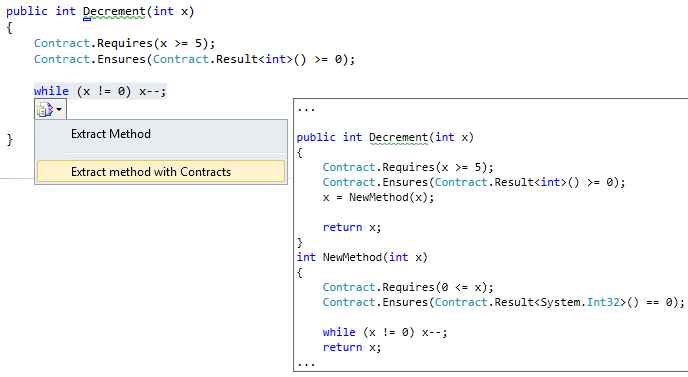
\includegraphics[width=\columnwidth]{2-RefactoredRoslyn}
\caption{A screenshot of the  extract method with contracts.
The suggested contract for the extracted method is  correct, safe, complete and the most general one.}
\label{ExtractMethodWithContracts}
\vspace{-0.5cm}
\end{figure}

\bibliographystyle{plain}
\bibliography{bib}

\end{document}

